% LAB 11: Web Scraping
%
% CSE/IT 107: Introduction to Programming
% New Mexico Tech
%
% Prepared by Russell White and Christopher Koch and Tyler Cecil
% Fall 2014
\documentclass[11pt]{cselabheader}
\usepackage{multicol,graphicx}

%%%%%%%%%%%%%%%%%% SET TITLES %%%%%%%%%%%%%%%%%%%%%%%%%
\fancyhead[R]{Lab 11: Web Scraping}
\title{Lab 11: Web Scraping}

\begin{document}

\maketitle

\hrule
\begin{quotation}
``The limits of my language mean the limits of my world.''
\end{quotation}
\begin{flushright}
--- Ludwig Wittgenstein
\end{flushright}

\begin{quotation}
``Any sufficiently advanced technology is indistinguishable from magic.''
\end{quotation}
\begin{flushright}
--- Arthur Clarke
\end{flushright}

\begin{quotation}
``Imagination is more important than knowledge.''
\end{quotation}
\begin{flushright}
--- Albert Einstein
\end{flushright}

\hrule

\section{Introduction}

In this lab, you will be extracting information from web pages and learning how
to plot some of it.

\section{HTML}

As you may be familiar, HTML is the main formatting language of the
Internet. HTML stands for HyperText Markup Language. As a language, it
defines where content appears on a website, and how it looks. For an
example, open up \texttt{Google Chrome} and navigate to
\texttt{http://www.nmt.edu}. Right click on the webpage, and select
``View Source''. What follows is the source code for \texttt{nmt.edu}!

HTML is actually fairly easy to read. All content exists between
various kinds of ``tags''. Each tag has a special kind of
meaning. Here is a simple example:

\begin{lstlisting}[style=python, language=html]
<html>
  <body>
    <p> This is a paragraph in the body of the page </p>
    <p> This text is <b> BOLD </b></p>
  </body>
</html>
\end{lstlisting}

To learn about all the various tags, see
\href{http://www.w3schools.com/}{W3Schools}.

\section{BeautifulSoup}

BeautifulSoup is a python library used to read HTML files in a nice
and easy way. In this lab, you will be using it along with urllib to
interact with Wikipedia pages.

Below is an example of a simple program using urllib. This
program gets a random Wikipedia article and prints out its URL. This
is identical to what would happen if you click on the Random Article button
on the Wikipedia homepage.

\lstinputlisting[style=python]{lab11/random_wikipage.py}

All of the logic for this program is inside the \lstinline{get_random}
function. First, it creates a \lstinline{Request} object. This is used
to tell urllib what page we want to load. First, we construct our URL using
the \lstinline{base} variable (since all of our URLs are going to start the
same way), then we pass a special headers argument. Don't worry too much about
what headers are -- in this case, we are only specifying a \lstinline{User-Agent}
string in order to identify ourselves to the remote server. We need to do this
because the default urllib \lstinline{User-Agent} string is blocked by
Wikipedia.

Once we have our \lstinline{Request} object created, we simply pass it to
\lstinline{request.urlopen} in order to get an object representing the page
we've loaded. Creating the \lstinline{Request} object and calling
\lstinline{request.urlopen} will be done no matter what page we are loading.

Once we have the page object, we simply check its URL (since the Wikipedia
random article button redirects you to a new page, this will not be the
same URL that we requested!) and strip off the beginning section, leaving
us with only /wiki/Article.

\pagebreak
\section{Matplotlib}

Matplotlib is a neat library for plotting in Python. It works similarly to
MATLAB plotting so that people with experience in that can easily switch over;
however, we will give you our own introduction to it.

Let's plot the following $x$ and $y$ coordinates:

\begin{table}[!ht]
  \centering
  \begin{tabular}{ llllllllllll }
    \bfseries x & 0 & 2 & 4 & 6 & 8 & 10 & 12 & 14 & 16 & 18\\
    \midrule
    \bfseries y & 0 & 4 & 8 & 12 & 16 & 20 & 24 & 28 & 32 & 36
  \end{tabular}
  \caption{Values for Figure~\ref{fig:x-2x}}
  \label{tab:x-2x}
\end{table}

\begin{lstlisting}[caption={Code to produce Figure~\ref{fig:x-2x}} with values from Table~\ref{tab:x-2x},label={lst:x-2x}]
import matplotlib.pylab as pl

x = range(0, 20, 2)
y = range(0, 40, 4)
pl.plot(x, y, '.')
pl.xlabel('X values')
pl.ylabel('Y values')
pl.title('Random plot of X vs Y')
pl.show()
\end{lstlisting}

\begin{figure}[!ht]
  \centering
  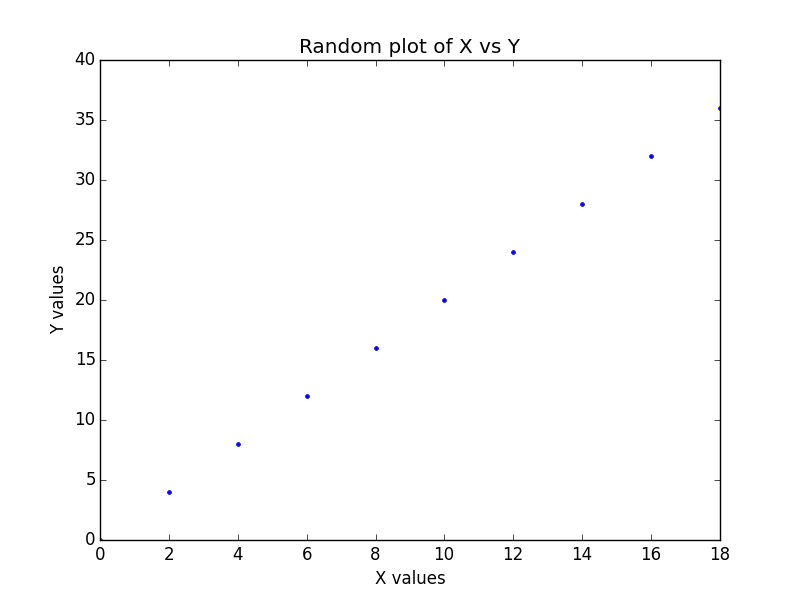
\includegraphics[width=0.8\textwidth]{lab11/x-2x-plot.png}
  \caption{Graph produced by Listing~\ref{lst:x-2x}}
  \label{fig:x-2x}
\end{figure}

The \lstinline!pl.plot()! function takes as arguments a sequence for x, a
sequence for y, and optionally a formatting specifier. The important ones are
``-'' for a solid line and ``.'' for point markers. You can add more options,
such as colors or labels. You can find more docs on
these specifiers on the Matploblib website:
\begin{center}
  \url{http://matplotlib.org/api/pyplot_api.html#matplotlib.pyplot.plot}
\end{center}

You have to call \lstinline!pl.show()! for the graph to actually show. There are
ways to print the graphs to image files, but we are not covering those for now.
You can look them up in the documentation if you want.

Bar plots work in a similar way. The \lstinline!pl.bar()! takes a sequence of
numbers to label the left side of the bars with and a sequence of heights of the
bars.

\begin{lstlisting}[caption={Code to produce Figure~\ref{fig:x-2x-bar}},label={lst:x-2x-bar}]
import matplotlib.pylab as pl

x = range(1, 11, 2)
y = range(1, 21, 4)
pl.bar(x, y)
pl.show()
\end{lstlisting}

\begin{figure}[!ht]
  \centering
  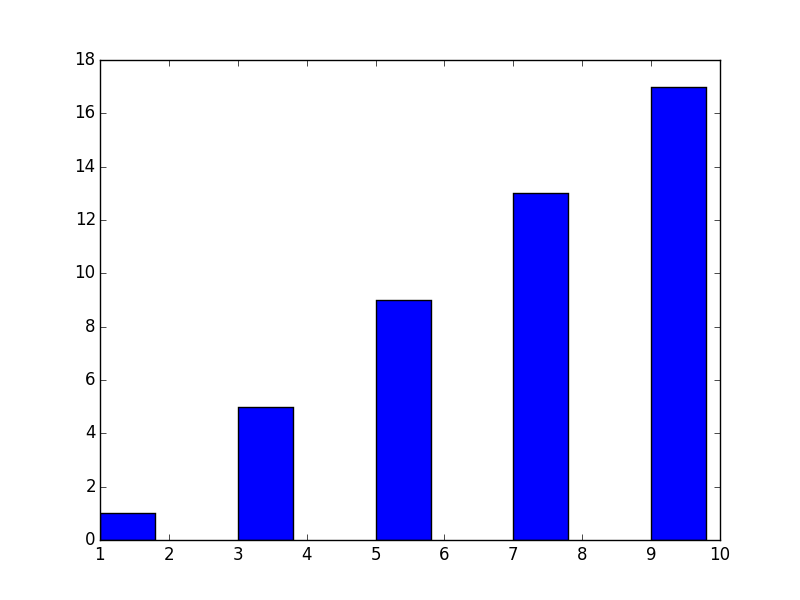
\includegraphics[width=0.8\textwidth]{lab11/x-2x-bar-plot.png}
  \caption{Graph produced by Listing~\ref{lst:x-2x-bar}}
  \label{fig:x-2x-bar}
\end{figure}

These are the two main functions you will need for plotting in this lab. If you
want to customize more, please see the matplotlib pylab documentation at
\begin{center}
  \url{http://matplotlib.org/api/pyplot_summary.html}
\end{center}

\pagebreak
\section{Wikipedia}

In case you feel like wasting time, did you know that wikipedia has some odd
properties about the philosophy page? You should read more at:

\centerline{\url{http://en.wikipedia.org/wiki/Wikipedia:Getting_to_Philosophy}.}

\pagebreak
\section{Exercises}
\label{sec:ex}

%One exerscis for soup (like get the title of a page)
%One for matplotlib (plot x^2)
%The main project

\begin{warningbox}{Boilerplate}
  Remember that this lab \emph{must} use the
  boilerplate syntax introduced in Lab~5.
\end{warningbox}

\begin{description}
  \item[file.py]
\end{description}

\pagebreak
\section{Submitting}

Files to submit:
\begin{itemize}
\item file.py (Section~\ref{sec:ex})
\end{itemize}

You may submit your code as either a tarball (instructions below) or as a .zip
file. Either one should contain all files used in the exercises for this lab.
The submitted file should be named either
\texttt{cse107\_firstname\_lastname\_lab11.zip} or
\texttt{cse107\_firstname\_lastname\_lab11.tar.gz} depending on which method you
used.

For Windows, use a tool you like to create a \texttt{.zip} file. The TCC
computers should have \texttt{7z} installed. For Linux, look at lab 1 for
instructions on how to create a tarball or use the ``Archive Manager'' graphical
tool.

\begin{center}
  \textbf{Upload your tarball or .zip file to Canvas.}
\end{center}

\end{document}
